\begin{frame}
\frametitle{What is NEXT?}

\begin{figure}[tbh!]
  \begin{center}
      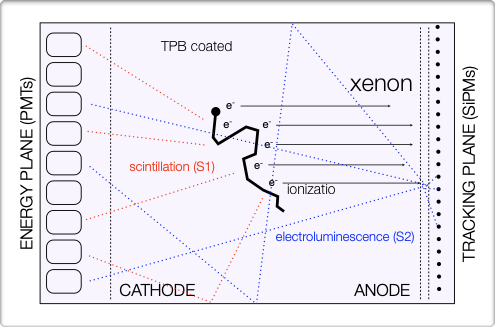
\includegraphics[width=0.45\textwidth]{moriond/next_poo.png}
       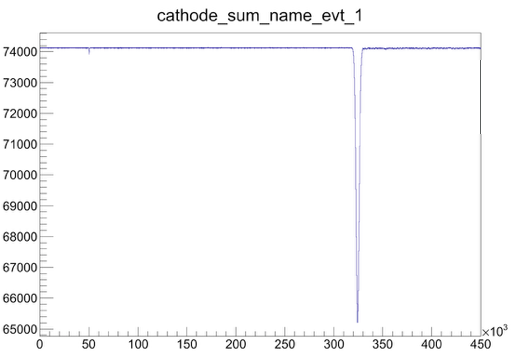
\includegraphics[width=0.45\textwidth]{moriond/next_s1_s2.png}      
  \end{center}
\end{figure}

\begin{itemize}
\item {\bf A HPXe:} High pressure gas chamber (10-20 bar) with EL amplification of the signal. 
\item {\bf Uses xenon,} a noble gas (source$ = $detector) with relatively high \Qbb\ and no long-lived radioactive isotopes. 
\item {\bf An optical TPC:} all signals are light. Primary scintillation (S1) gives \tz\ (needed to fiducialize the event and to correct for finite electron lifetime), EL amplification gives S2, which is used to measure energy and to reconstruct the electron trajectory. 
\end{itemize}
\end{frame}

\begin{frame}
\frametitle{NEXT assets}
\begin{figure}[tbh!]
  \begin{center}
      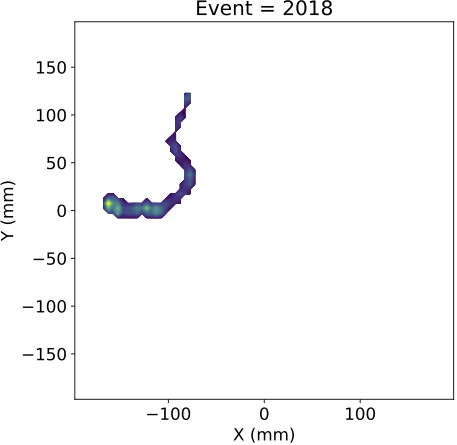
\includegraphics[width=0.20\textwidth]{moriond/single_e.png}
      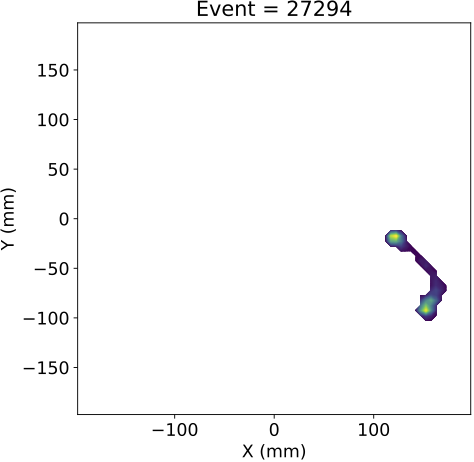
\includegraphics[width=0.20\textwidth]{moriond/double_e.png}
  \end{center}
 \end{figure}
  
 \begin{figure}[tbh!]
  \begin{center}
      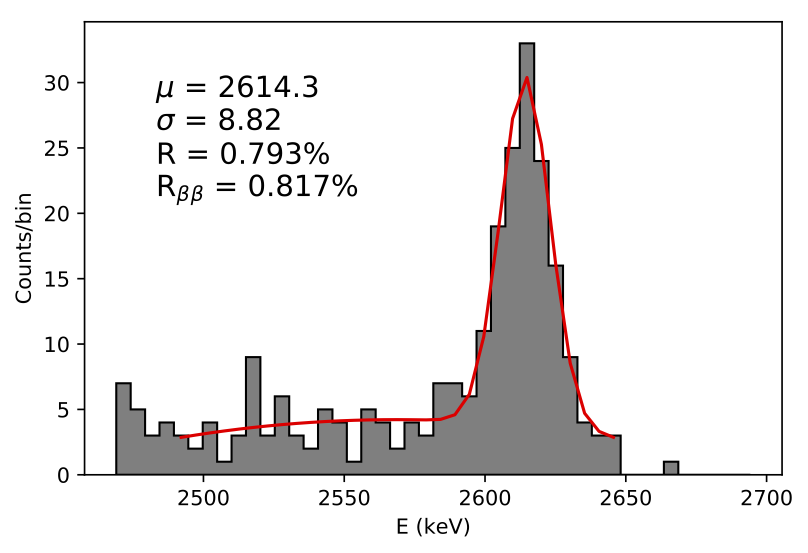
\includegraphics[width=0.25\textwidth]{moriond/CSTH_espectrum_Tl_photopeak_fit.png}
       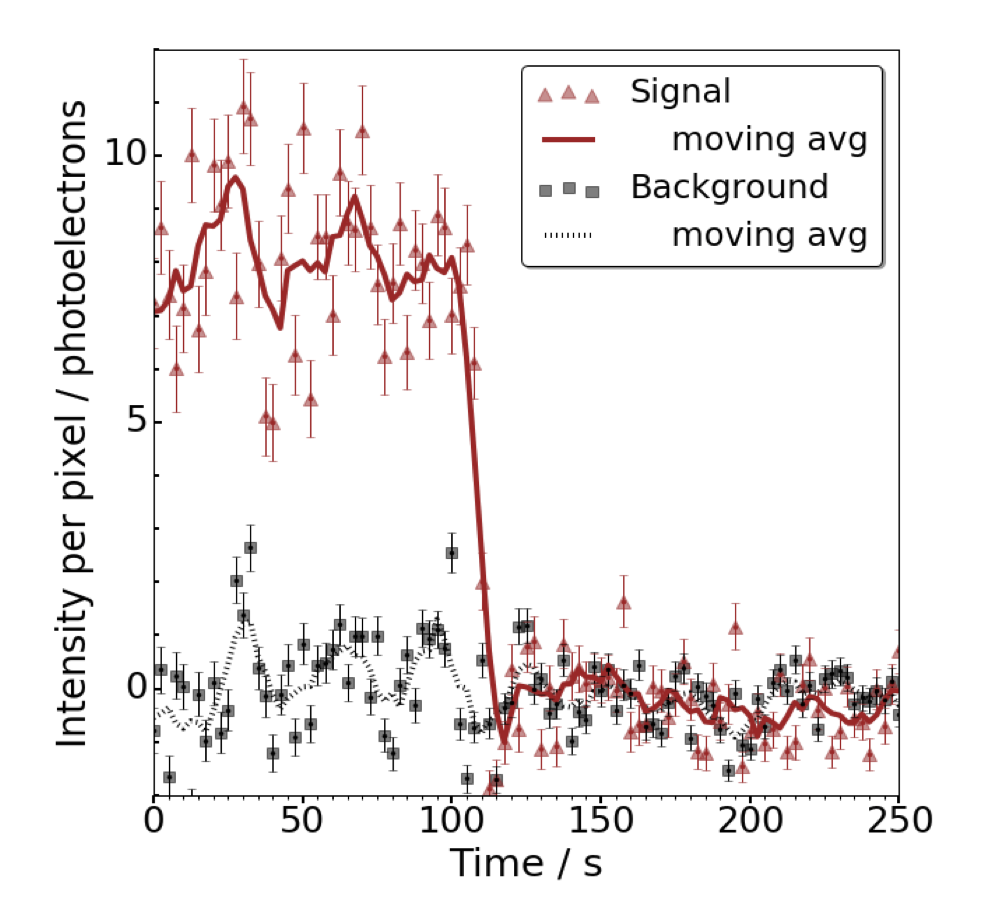
\includegraphics[width=0.20\textwidth]{moriond/smfi_trayectory.png}    
  \end{center}
 \end{figure}

 
\begin{itemize}
\item {\bf Topological signal}, capable to separate signal ``double electrons'', from backgrounds ``single electrons''. 
\item {\bf Excellent energy resolution}, 20 keV at \Qbb. 
\item {\bf Possibility to identify \Bapp} produced in $\XE \rightarrow \Bapp + 2 e (+ 2 \nu)$, through SMFI. 
\end{itemize}
\end{frame}


\begin{frame}
\frametitle{The NEXT program} 
 \begin{center}
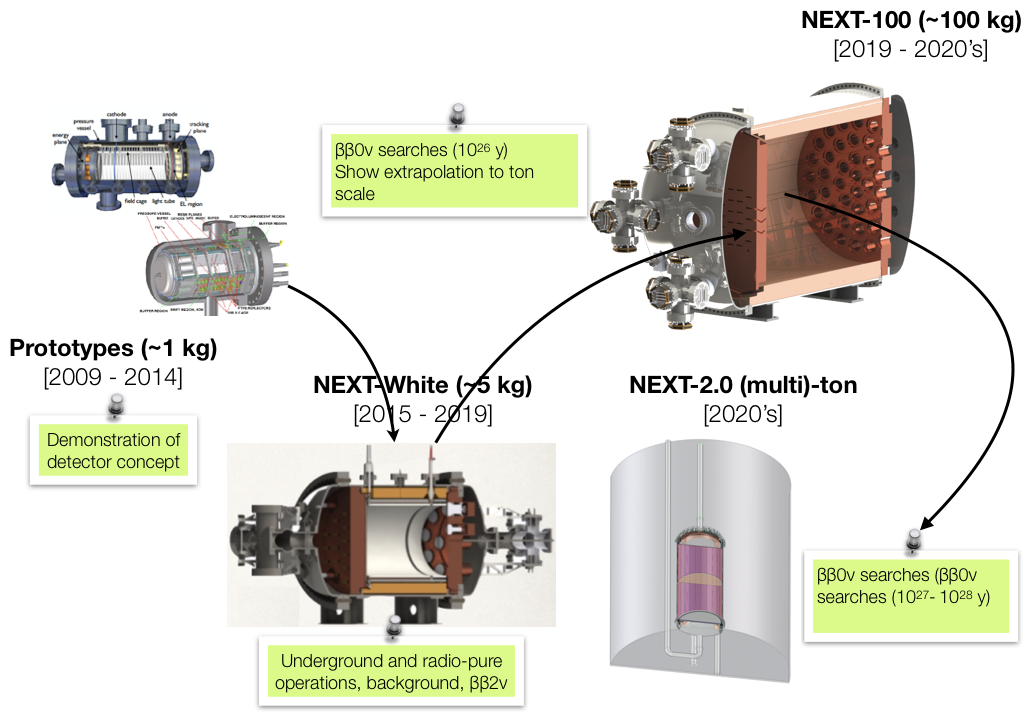
\includegraphics[width=0.85\textwidth]{moriond/next-program.png}
\end{center}
\end{frame}



